\documentclass[pdflatex,sn-mathphys-num]{sn-jnl}

\usepackage{graphicx}
\usepackage{multirow}
\usepackage{amsmath,amssymb,amsfonts}
\usepackage{booktabs}
\usepackage{url}

\begin{document}

\title[GraphPSS: a protein contact graph benchmark]{GraphPSS: A Large-Scale Protein Contact Graph Benchmark for Node Classification}

\author*[1]{\fnm{Alireza} \sur{Hashemi}}\email{ahashemi@gradcenter.cuny.edu}

\affil*[1]{\orgname{CUNY The Graduate Center}, \orgaddress{\city{New York}, \state{NY}, \country{USA}}}

\abstract{Node classification benchmarks are dominated by small single-graph citation networks. We introduce GraphPSS, an inductive benchmark of 172,891 protein contact graphs with 54 million nodes, built from the Protein Data Bank. The task is to classify each residue as helix, sheet, or coil from the contact graph alone, and a homology-aware split keeps proteins from related families apart. We provide a standard protocol and baselines from seven graph neural networks (GNNs), gradient-boosted trees, and simpler methods. A compact graph attention model, PSS-net, reaches 91.02$\pm$0.03\% accuracy with 1.7M parameters, against 87.1\% for trees on hand-crafted contact features and 78.4\% for the same input without message passing. Three lessons for graph learning follow. Graph models can be misjudged when leakage is ignored: a random split inflates GNN accuracy by 3.3--6.5 points but trees by only 0.7, and changes their ranking. Node input design matters more than architecture in this setting: a translation-invariant input built from contact separations adds 6--7 points over a positional embedding for every architecture tested, and a poor input can make attention collapse to the majority class. Finally, expanding the neighborhood of a graph convolution adds 3.4--3.6 points over GCN. GraphPSS offers a large, label-rich task where such effects can be measured.}

\keywords{Graph neural networks, Benchmark dataset, Node classification, Data leakage, Protein contact maps, Graph attention}

\maketitle

\section{Introduction}\label{sec:intro}

Benchmarks shape which graph learning methods appear to work. Node classification research has long relied on single-graph citation networks such as Cora~\cite{cora}, Citeseer~\cite{citeseer}, and PubMed~\cite{pubmed}, which are small and transductive. The Open Graph Benchmark~\cite{hu2020open} and multi-graph datasets such as PPI~\cite{hamilton2017sage} address scale and inductive learning, but large inductive node-level tasks over many small graphs, with labels that have a physical meaning, remain rare.

We introduce GraphPSS (\textbf{Graph} \textbf{P}rotein \textbf{S}econdary \textbf{S}tructure), a dataset of contact graphs for 172,891 proteins from the Protein Data Bank (PDB)~\cite{pdb}. Each graph connects residues that are close in space, and each node is labeled as helix, sheet, or coil. Amino-acid types and coordinates are withheld, so the task rests on graph structure alone. Proteins also fall into evolutionary families, which gives the dataset a natural notion of related samples and allows a direct measurement of how much a model relies on near-duplicates in training data.

This is a benchmark paper. The task is a controlled test for graph learning, and it is not a replacement for tools that assign secondary structure from coordinates. Because the labels derive from the same 3D structure as the graphs, our accuracies should not be compared with those of sequence-based predictors.

Our contributions are:
\begin{itemize}
    \item \textbf{A dataset.} GraphPSS has 173K graphs and 54M nodes, with a script that regenerates it from PDB files and a documented label definition.
    \item \textbf{A protocol.} We define a homology-aware split based on 30\% sequence-identity clusters, together with evaluation rules.
    \item \textbf{Baselines.} We report results for seven GNNs with an equal hyper-parameter sweep and for non-GNN baselines. The best model is PSS-net, a compact attention model with 1.7M parameters.
    \item \textbf{Lessons for graph learning.} We quantify homology leakage, show that node input design outweighs architecture, explain a symmetry failure of attention under uninformative inputs, and show the benefit of an expanded neighborhood.
\end{itemize}

\section{Related Work}\label{sec:related}

\paragraph{Graph benchmarks.} Citation networks~\cite{cora,citeseer,pubmed} and the knowledge graph NELL~\cite{Carlson_Betteridge_Kisiel_Settles_Hruschka_Mitchell_2010} remain common for node classification. Protein contact maps have been used as graph data, for example in D\&D~\cite{10.1093/bioinformatics/bti1007}, but with under 1,200 graphs and for graph-level labels. Table~\ref{tab:datasets} compares these datasets.

\paragraph{Leakage.} Leakage between training and test data is a known cause of over-optimistic results across machine learning~\cite{kapoor2023leakage}. In protein data, homologs are the main source, and we measure its effect on graph models.

\paragraph{Secondary structure.} Most deep learning work predicts secondary structure from sequence~\cite{deepcnf,jpred,pssp}, and one study combines sequence embeddings with GNNs on a small PDB subset~\cite{pssgnn}. These address a different problem. Closer to ours, P-SEA~\cite{labesse1997psea} and PCASSO~\cite{law2014pcasso} assign secondary structure from C$\alpha$ coordinates, the latter reporting about 95\% agreement with DSSP~\cite{dssp}. Coordinates carry more information than a binary contact graph, so these are the better practical tools when coordinates exist. Since they target DSSP and our labels are PDB records, the numbers are not directly comparable.

\begin{table}[t]
\caption{GraphPSS compared with commonly used graph datasets. D\&D is included because it also consists of protein contact maps.}
\label{tab:datasets}
\begin{tabular}{lrrl}
\toprule
Dataset & Graphs & Nodes & Classes \\
\midrule
Cora & 1 & 2,708 & 7 (node) \\
Citeseer & 1 & 3,327 & 6 (node) \\
PubMed & 1 & 19,717 & 3 (node) \\
NELL & 1 & 65,755 & 210 (node) \\
D\&D & 1,178 & 334K & 2 (graph) \\
GraphPSS & 172,891 & 54.2M & 3 (node) \\
\botrule
\end{tabular}
\end{table}

\section{The GraphPSS Dataset}\label{sec:dataset}

\subsection{Background}

Proteins are chains of amino-acids. Secondary structure is the local shape of the chain, stabilized by hydrogen bonds between backbone groups~\cite{pauling1951structure}. In a helix, residue $i$ bonds with residue $i+4$, and the chain coils. In a strand, the chain is extended, and strands pair into sheets through bonds that can join residues far apart in the sequence. Other residues are grouped as coil.

These shapes leave signatures in a contact graph. Consecutive C$\alpha$ atoms are about 3.8 \AA{} apart. In a helix, residues $i$ and $i+3$ are about 5 \AA{} apart and $i$ and $i+4$ about 6 \AA{}, so both are contacts at 8 \AA{}, while in an extended strand $i$ and $i+3$ are about 10 \AA{} apart and are not. Paired strands instead produce bands of long-range contacts. Local patterns thus identify helices, and sheets require information from distant residues, so the task needs message passing.

\begin{figure}[t]
\centering
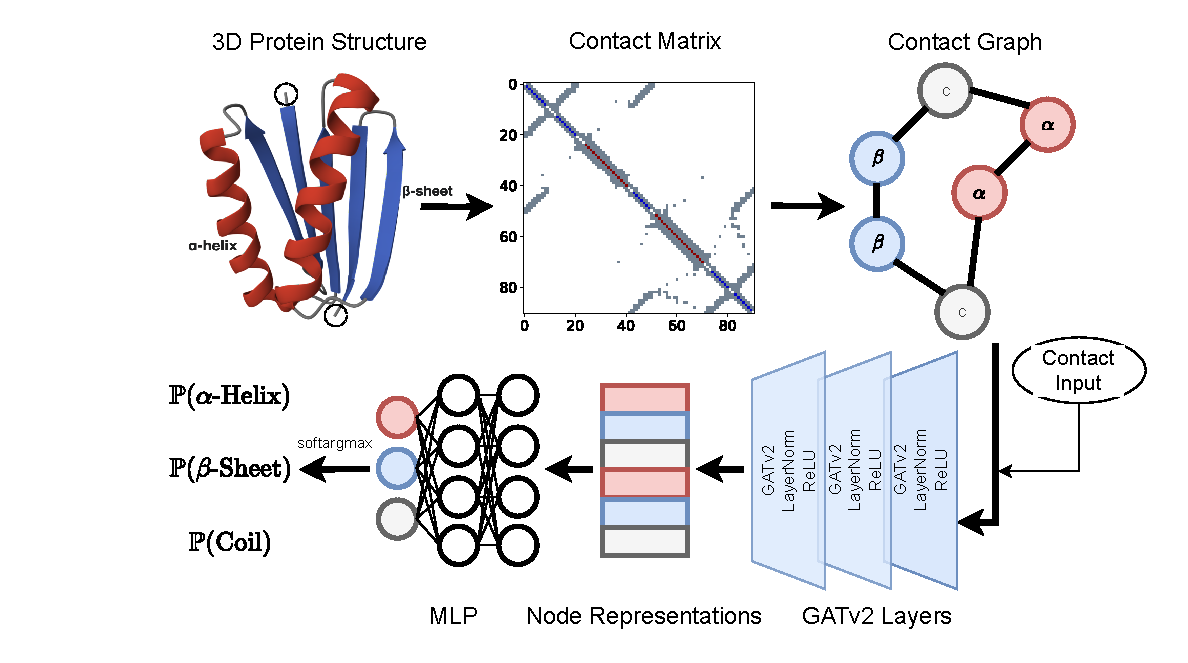
\includegraphics[width=0.95\textwidth]{flow.pdf}
\caption{From protein to benchmark task, for a sample protein (1QYS) with 91 observed residues. The contact matrix (grey) shows the node classes on its diagonal: helices in red, sheets in blue, and coils in white. A GNN and an MLP map the contact graph and the node input of Section~\ref{sec:input} to class probabilities. The number of layers drawn is schematic.}
\label{fig:flow}
\end{figure}

\subsection{Construction}

The PDB held about 214,000 entries when it was downloaded in late 2023, including structures that are not proteins. For each entry we take the first chain of the first model and keep its C$\alpha$ atoms as nodes. Two residues are connected if their C$\alpha$ atoms are closer than 8 \AA, a widely used contact threshold~\cite{park2000toward,gnn-prot}. Fig.~\ref{fig:flow} shows the process. Processing gave graphs for 173,182 entries, and removing the 291 with 2,000 or more residues leaves 172,891. No filter on experimental method or resolution was applied.

Labels are the secondary structure records of the PDB files: a residue is helix if it lies within a helix range (\texttt{\_struct\_conf}), sheet if within a sheet range (\texttt{\_struct\_sheet\_range}), and coil otherwise. These are not DSSP output. Our script reproduces the stored graphs exactly and 99.999\% of stored labels on 299 randomly chosen proteins. The labels agree with DSSP on 93.0\% of residues on 294 of these proteins, under the mapping of H, G, and I to helix and E to sheet.

\subsection{Statistics}

The dataset has 54,186,863 nodes and 531 million directed edges, with a mean degree of 9.8. The median graph has 271 residues and the largest has 1,997 (Fig.~\ref{fig:dist}). Of the nodes, 42.2\% are helix, 36.4\% coil, and 21.4\% sheet. Almost all graphs (99.0\%) are connected. Residue indices count observed residues, so a sequence separation across an unresolved segment is smaller than the true one; 36.6\% of chains in a sample of 993 have such a gap.

\begin{figure}[t]
\centering
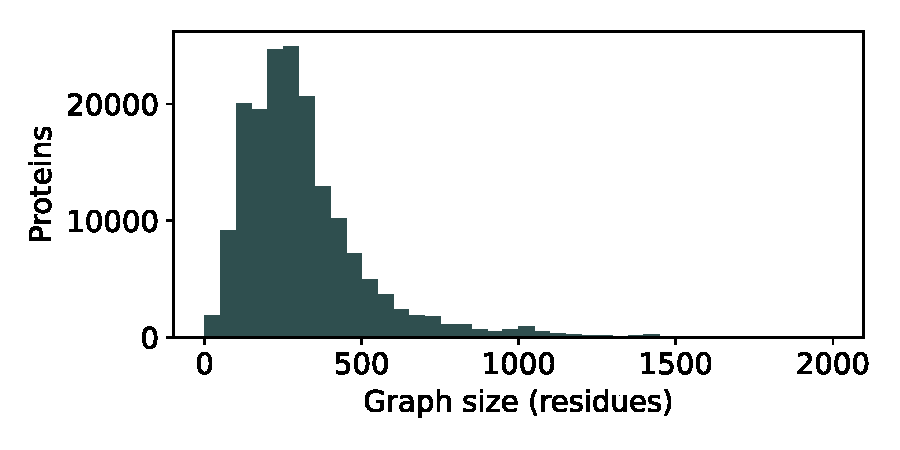
\includegraphics[width=0.48\textwidth]{figures/dist_sizes.pdf}
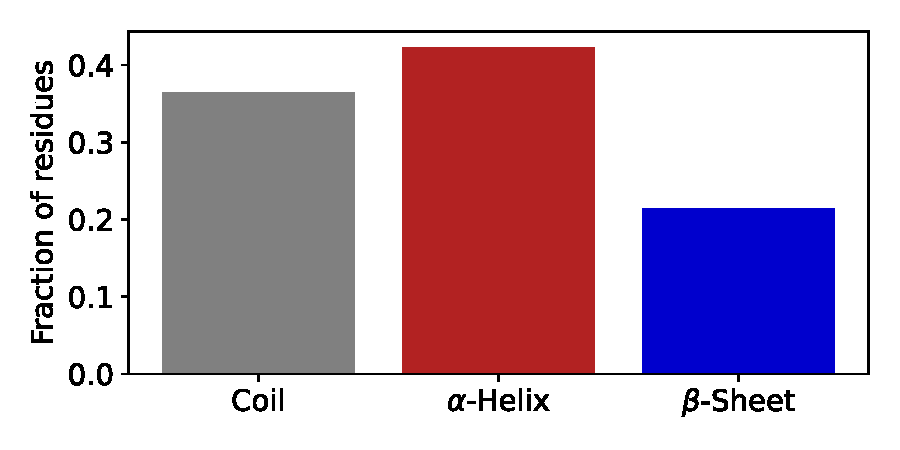
\includegraphics[width=0.48\textwidth]{figures/dist_labels.pdf}
\caption{Distribution of graph sizes (left) and node labels (right).}
\label{fig:dist}
\end{figure}

\subsection{Availability, Maintenance, and Responsible Use}

The graphs and splits are available on Zenodo at \url{https://doi.org/10.5281/zenodo.23829544}, and the code, splits, and per-run results at \url{https://github.com/ialireza13/graphpss}. This release is a fixed snapshot, so that results stay comparable. The graph builder can regenerate samples from current PDB files, but remediation of the archive can change individual entries, so comparisons should use the released version. Issues and corrections are tracked on GitHub.

PDB records come from different depositors and software, so the labels are less uniform than those of a single assignment program, and users should not treat them as ground truth for structural biology. Models trained here should not be used to replace coordinate-based assignment, and their accuracies should not be reported as sequence-based prediction. The dataset contains public structural data of macromolecules and no personal data.

\section{Benchmark Protocol}\label{sec:protocol}

\paragraph{Task.} Given a contact graph, predict the class of every node. The task is inductive, since test graphs are unseen. Models may use only the graph and the order of residues along the chain, not amino-acid types or coordinates.

\paragraph{Splits.} The main split keeps homologs apart. Each entry is assigned to the RCSB sequence cluster at 30\% identity, computed with MMseqs2~\cite{steinegger2017mmseqs2}, of the chain its graph was built from, a level below which alignments become unreliable as evidence of homology~\cite{rost1999twilight}. Whole clusters are assigned to train, validation, and test, reaching 80/10/10\% of residues. This gives 21,700 groups, the largest holding 1.6\% of residues, and 137,636 training, 17,385 validation, and 17,870 test graphs. The share of test proteins with a sequence identical to that of a training protein falls from 16.9\% under a random split to 0.9\%. A random 80/10/10\% split by entry is also provided, only for measuring leakage.

\paragraph{Metrics.} We report residue accuracy (Q3, the standard measure for this task), macro-F1 for class imbalance, and mean per-protein accuracy so that large proteins do not dominate. Results should be reported over at least 3 seeds.

\paragraph{Rules.} Hyper-parameters and early stopping use the validation set only, and the test set is evaluated once. Results should state the node input and the parameter count. Results on the random split should not be reported as the main result.

\section{Models and Baselines}\label{sec:models}

\subsection{Node Input}\label{sec:input}

Contact graphs have no node attributes, so a model needs a node input. A common choice is a learned embedding of the node's position in the chain. This forces the model to infer sequence separations from pairs of embeddings, and it allows memorizing absolute positions.

We propose a translation-invariant input. Let $s_{ij} = \mathrm{clip}(j - i, -R, R)$ be the clipped sequence separation of a contact, with $R=16$. Each residue starts from
\begin{equation}
    h_i^{(0)} = c + \sum_{j \in N(i)} e(s_{ij}),
\end{equation}
where $e$ is a learned 32-dimensional embedding and $c$ a learned constant. For GAT and GATv2 layers, each edge also carries a 16-dimensional embedding of $s_{ij}$.

Both parts are needed. GAT layers use edge features only in the attention coefficients, not in the messages. With identical node inputs, a weighted mean of neighbors is the same vector for every node, so all nodes stay identical whatever the edge features are. A GATv2 model with separation edge features and constant node inputs indeed collapses to the majority class (41.1\%).

\subsection{Architectures}

Every model has the node input, a stack of GNN layers, each followed by layer normalization and ReLU, and a fully connected head. We compare GCN~\cite{kipf2017semisupervised}, GIN~\cite{xu2019powerful} with a 3-layer MLP, GraphSAGE~\cite{hamilton2017sage} with mean aggregation, GAT~\cite{veličković2018graph}, GATv2~\cite{brody2022attentivegraphattentionnetworks}, and the expanded GCN~\cite{hashemi2024visiting}.

The expanded GCN lets each layer see beyond direct neighbors. Let $A_k$ connect node pairs at shortest-path distance exactly $k$, with $A_0 = I$, and let $D_k$ be its degree matrix. A layer of order $K$ is
\begin{equation}
    H^{(l+1)} = \sigma\Big( \sum_{k=0}^{K} \gamma_k^{(l)} D_k^{-1} A_k H^{(l)} W^{(l)} + b^{(l)} \Big),
\end{equation}
where $\gamma^{(l)}$ is learned per layer. We use $K \in \{2,3\}$.

For GATv2, with edge features $z_{ij}$,
\begin{align}
    h_v^{(l+1)} &= \sigma\Big( \sum_{u \in N(v) \cup \{v\}} \alpha_{vu} W^{(l)} h_u^{(l)} \Big), \\
    \alpha_{ij} &= \underset{j \in N(i) \cup \{i\}}{\mathrm{softmax}} \, \mathbf{a}^\top \mathrm{LeakyReLU}\big( W_1 h_i + W_2 h_j + W_3 z_{ij} \big).
\end{align}

PSS-net is the GATv2 model selected by the sweep: the node input above, 4 layers with 4 heads of size 128, and a head that maps the 512-dimensional representations to 128 dimensions and then to 3 logits. It has 1.72M parameters.

\subsection{Training and Selection}

Models are trained with cross-entropy and Adam~\cite{kingma2017adammethodstochasticoptimization}, with batches of 32 proteins, gradient clipping at 1.0, and cosine annealing~\cite{loshchilov2017sgdrstochasticgradientdescent} of the learning rate from $10^{-3}$ to $10^{-4}$. Training runs for at most 20 epochs and stops when the validation loss has not improved for 5 epochs, and the checkpoint with the best validation loss is evaluated once on the test set. We used PyTorch 2.5~\cite{paszke2019pytorch} and PyTorch Geometric 2.6 with bf16 mixed precision on one NVIDIA A100 GPU.

Each architecture gets the same sweep of 38 runs in total (Table~\ref{tab:sweep}), on 25\% of the training proteins for 10 epochs. The configuration with the best validation accuracy per architecture is retrained on the full training set with seeds 0, 1, and 2. GAT was run with one seed as a side comparison.

\begin{table}[t]
\caption{Hyper-parameter sweep. Width is the per-node dimension after a layer, which for attention models is heads times per-head size. GAT was run with 2 and 3 layers at width 2048 only.}
\label{tab:sweep}
\begin{tabular}{ll}
\toprule
Parameter & Values \\
\midrule
Layers & 2, 3, 4 \\
Width & 512, 2048 \\
Attention heads (GAT, GATv2) & 4 \\
Neighborhood order (expanded GCN) & 2, 3 \\
\botrule
\end{tabular}
\end{table}

\subsection{Non-GNN Baselines}

\begin{itemize}
    \item \textbf{Gradient-boosted trees.} Histogram gradient boosting~\cite{pedregosa2011sklearn} on contacts at each separation up to $\pm R$, long-range contact count, degree, relative position, and chain length, for the residue and its neighbors at $\pm1$ and $\pm2$, with $R \in \{8, 16\}$. It is trained on 20,000 proteins to keep training practical. Accuracy at $R=8$ rose only from 86.3\% to 86.4\% between 2,000 and 20,000 proteins, so more data is unlikely to close the gap to the best GNNs.
    \item \textbf{Contact MLP.} The contact-separation input with an MLP per residue and no message passing.
    \item \textbf{Contact rule.} A fixed rule built from the helix and strand signatures above, with no training.
    \item \textbf{Spectral clustering}~\cite{sc} on the normalized Laplacian, with clusters matched to classes per graph by the Hungarian algorithm~\cite{kuhn}. Matching uses true labels, so this is an optimistic bound. It was run on 2,000 test proteins.
    \item \textbf{Position MLP and majority class.} An MLP on the position embedding, and the most frequent class.
\end{itemize}

\section{Results}\label{sec:results}

\subsection{Baseline Results}

Table~\ref{tab:main} gives the reference results. PSS-net is the most accurate, at 91.02$\pm$0.03\%, and it is the smallest of the selected models. GAT and GraphSAGE follow. All three beat the trees, which reach 87.1\% with the same $\pm16$ contact information, while GCN and GIN fall below them. Message passing adds about 13 points over a residue's own contact profile, and the residue position alone stays close to the majority class. The attention models also have edge features that the others lack, so this comparison does not isolate attention from edge features. In the sweep, one GIN configuration (4 layers, width 2048) diverged to the majority class.

\begin{sidewaystable}
\caption{Reference results on the test set of the homology-aware split, in percentages. Mean$\pm$standard deviation over 3 seeds where shown. $^\dagger$One seed. $^\ddagger$2,000 proteins, with oracle matching of clusters to classes.}
\label{tab:main}
\begin{tabular}{llrcccc}
\toprule
Model & Layers $\times$ width & Params & Test Q3 & Per-protein acc. & Macro-F1 & F1 coil / helix / sheet \\
\midrule
\textbf{PSS-net (GATv2)} & $4 \times 512$ & 1.72M & \textbf{91.02$\pm$0.03} & \textbf{91.35$\pm$0.04} & \textbf{90.82$\pm$0.05} & 87.7 / 94.1 / 90.6 \\
GAT$^\dagger$ & $3 \times 2048$ & 9.64M & 90.83 & 91.15 & 90.61 & 87.5 / 94.1 / 90.2 \\
GraphSAGE & $4 \times 2048$ & 29.5M & 90.07$\pm$0.05 & 90.49$\pm$0.06 & 89.83$\pm$0.05 & 86.6 / 93.6 / 89.3 \\
Expanded GCN ($K=3$) & $4 \times 2048$ & 16.9M & 89.70$\pm$0.05 & 90.09$\pm$0.04 & 89.41$\pm$0.04 & 86.0 / 93.4 / 88.8 \\
Expanded GCN ($K=2$) & $4 \times 2048$ & 16.9M & 89.53$\pm$0.08 & 89.96$\pm$0.07 & 89.24$\pm$0.10 & 85.8 / 93.3 / 88.6 \\
Gradient-boosted trees ($R=16$) & -- & -- & 87.07 & 87.25 & 86.36 & 82.5 / 93.0 / 83.6 \\
Gradient-boosted trees ($R=8$) & -- & -- & 86.42 & 86.62 & 85.62 & 81.6 / 92.9 / 82.4 \\
GCN & $2 \times 2048$ & 8.5M & 86.12$\pm$0.11 & 86.75$\pm$0.11 & 85.68$\pm$0.11 & 81.5 / 91.2 / 84.4 \\
GIN & $2 \times 2048$ & 37.9M & 85.87$\pm$0.19 & 86.42$\pm$0.20 & 85.43$\pm$0.21 & 81.2 / 91.1 / 84.0 \\
Contact MLP & $3 \times 2048$ & 8.5M & 78.36$\pm$0.01 & 78.26$\pm$0.01 & 76.99$\pm$0.01 & 71.6 / 87.4 / 72.0 \\
Contact rule & -- & -- & 65.28 & 65.11 & 59.98 & 35.2 / 79.2 / 65.6 \\
Spectral clustering$^\ddagger$ & -- & -- & 44.5 & -- & -- & -- \\
Position MLP & $3 \times 2048$ & 8.5M & 41.86 & 40.47 & 24.04 & 14.1 / 58.1 / 0.0 \\
Majority class & -- & -- & 41.10 & 39.31 & 19.42 & 0.0 / 58.3 / 0.0 \\
\botrule
\end{tabular}
\end{sidewaystable}

The expanded GCN improves on GCN by 3.4 points with $K=2$ and 3.6 with $K=3$, well above the seed-level standard deviation of about 0.1, and approaches GraphSAGE.

\subsection{Model Efficiency}

Fig.~\ref{fig:eff} shows the accuracy and size of all sweep runs. Attention models lie above the others at every size. The smallest GATv2 model, with 0.65M parameters, reaches 90.16\% validation accuracy, more than any non-attention model at any size: the best of these is GraphSAGE at 89.63\% with 29.5M parameters, about 45 times more. Width also adds nothing to GATv2: with 4 layers, 1.72M parameters give 90.89\%, and 26.5M give 90.86\%. This advantage is in parameters and not in training time, since attention costs more per parameter: a final PSS-net run took 1.3 hours, against 0.5 for GraphSAGE and 0.8 for GCN.

\begin{figure}[t]
\centering
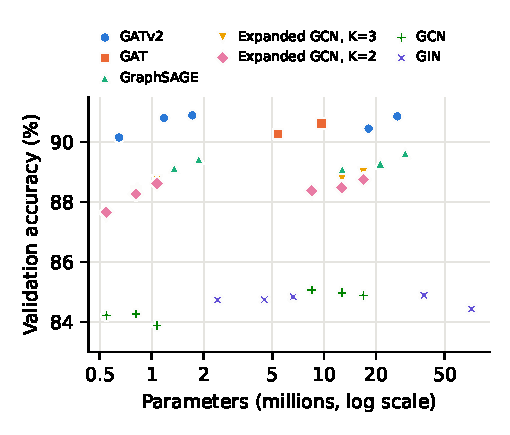
\includegraphics[width=0.6\textwidth]{figures/efficiency.pdf}
\caption{Validation accuracy against number of parameters for the sweep runs, trained on 25\% of the training proteins for 10 epochs. One diverged GIN run (41.7\%) is outside the axis.}
\label{fig:eff}
\end{figure}

\subsection{Effect of Node Input}

Table~\ref{tab:input} compares the contact-separation input with a learned embedding of the absolute residue index at the same model settings. The contact input adds 5.8--7.2 points for all three architectures, more than the gap between most architectures. The settings were selected with the contact input, so the position models were not tuned separately, but a separate 12-epoch run of GATv2 with 2 layers reached a similar 84.05\%.

\begin{table}[t]
\caption{Test accuracy on the homology-aware split with the contact-separation input and with an embedding of the absolute residue index (seed 0).}
\label{tab:input}
\begin{tabular}{lccc}
\toprule
Model & Contact input & Absolute index & Gain \\
\midrule
GATv2 & 91.05 & 84.63 & +6.4 \\
Expanded GCN ($K=2$) & 89.47 & 82.24 & +7.2 \\
GCN & 86.04 & 80.28 & +5.8 \\
\botrule
\end{tabular}
\end{table}

\subsection{Homology Leakage}

Table~\ref{tab:leak} compares the two splits. GNNs gain 3.3--6.5 points from the random split, while the trees, which see only local contact features, gain 0.7. GNNs therefore partly exploit similarity to training proteins, and the gain is largest for the weakest model. This changes conclusions: a random split places GCN 5.4 points above the trees, while on the homology-aware split it is 0.4 points below them at $R=8$.

\begin{table}[t]
\caption{Test accuracy on the homology-aware and random splits (seed 0).}
\label{tab:leak}
\begin{tabular}{lccc}
\toprule
Model & Homology-aware & Random & Gain \\
\midrule
PSS-net (GATv2) & 91.05 & 94.36 & +3.3 \\
Expanded GCN ($K=2$) & 89.47 & 94.14 & +4.7 \\
GCN & 86.04 & 92.54 & +6.5 \\
Gradient-boosted trees ($R=8$) & 86.42 & 87.13 & +0.7 \\
\botrule
\end{tabular}
\end{table}

\subsection{Robustness to Edge Perturbation}

We evaluate trained models on perturbed test graphs, without retraining (Table~\ref{tab:robust}), by dropping contacts with $|i-j| \geq 3$ or adding random ones. All models tolerate spurious edges, with attention models losing the least: 2.3 points when 25\% are added, against 5.9 for GCN. None tolerates missing edges. Dropping 10\% costs 5--9 points, and dropping all of them leaves 36.6\%, since the $i \pm 3$ and $i \pm 4$ contacts that identify helices are among those removed. GATv2 falls fastest at 25\%, which is consistent with its attention pattern below.

\begin{table}[t]
\caption{Test accuracy when a percentage of contacts with $|i-j| \geq 3$ is dropped, or the same percentage of random ones added (seed 0).}
\label{tab:robust}
\begin{tabular}{lccccc}
\toprule
Model & Clean & Drop 10 & Drop 25 & Add 10 & Add 25 \\
\midrule
GATv2 & 91.1 & 82.5 & 63.3 & 90.3 & 88.8 \\
GAT & 90.8 & 83.2 & 65.3 & 90.1 & 88.5 \\
GraphSAGE & 90.1 & 82.5 & 65.0 & 89.1 & 86.7 \\
Expanded GCN ($K=3$) & 89.7 & 82.2 & 67.4 & 88.7 & 86.9 \\
GCN & 86.0 & 79.5 & 66.4 & 83.9 & 80.1 \\
GIN & 86.0 & 80.5 & 68.9 & 83.9 & 80.2 \\
Contact MLP & 78.4 & 72.9 & 63.6 & 77.4 & 76.0 \\
\botrule
\end{tabular}
\end{table}

\subsection{Error Analysis}

Table~\ref{tab:conf} shows the confusion matrix of PSS-net. Most errors involve coil, while helix and sheet are almost never confused (0.2--0.3\%). Errors concentrate at segment boundaries: residues adjacent to a change of class are 27.4\% of all residues but 56.7\% of errors, with 81.5\% accuracy against 96.0\% for residues at least 3 positions from a boundary (Fig.~\ref{fig:sample}). A segment counts as found when most of its residues are correct. Helices of 7 or more residues are found 98--100\% of the time, against 74\% for 4--6 residues and 65\% for 1--3, and strands of 4 or more residues 99\% of the time, against 85\% for 1--3. Per-protein accuracy has a median of 91.9\% and a 5th percentile of 83.3\%, and it is stable for chains from 50 to 2,000 residues (89.5--92.0\%), and lower below 50 (83.1\%).

The last GATv2 layer places 87.2\% of its attention on pairs with $|i-j| \leq 4$, self-loops included, while these pairs are 62.6\% of edges (Fig.~\ref{fig:att}). The model has thus learned to focus on the short-range contacts that define local structure, which also explains its sensitivity to removing them.

\begin{table}[t]
\caption{Confusion matrix of PSS-net on the test set, as percentages of each true class (seed 0, 5.4M residues).}
\label{tab:conf}
\begin{tabular}{lccc}
\toprule
True \textbackslash{} Predicted & Coil & Helix & Sheet \\
\midrule
Coil & 86.9 & 6.7 & 6.4 \\
Helix & 5.5 & 94.3 & 0.2 \\
Sheet & 7.8 & 0.3 & 92.0 \\
\botrule
\end{tabular}
\end{table}

\begin{figure}[t]
\centering
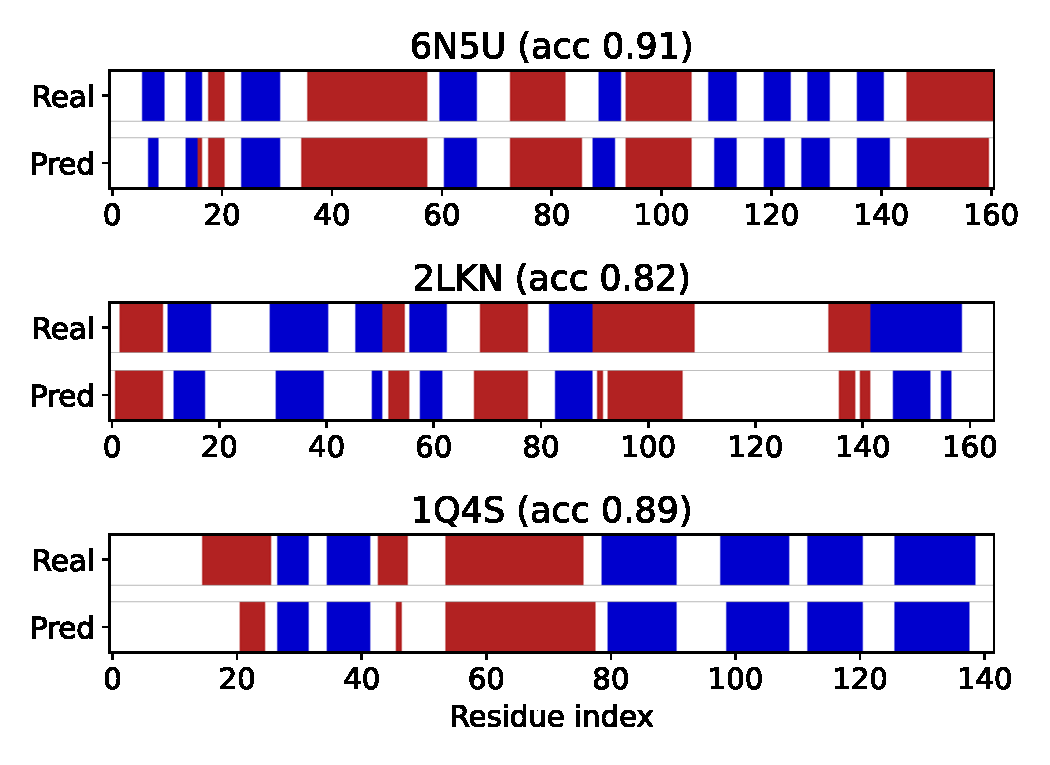
\includegraphics[width=0.7\textwidth]{figures/sample.pdf}
\caption{True (upper band) and predicted (lower band) classes for test proteins 6N5U, 2LKN, and 1Q4S, with helices in red, sheets in blue, and coils in white. The proteins were chosen at random from the test set among chains of 100--180 residues with at least 20\% helix and 20\% sheet.}
\label{fig:sample}
\end{figure}

\begin{figure}[t]
\centering
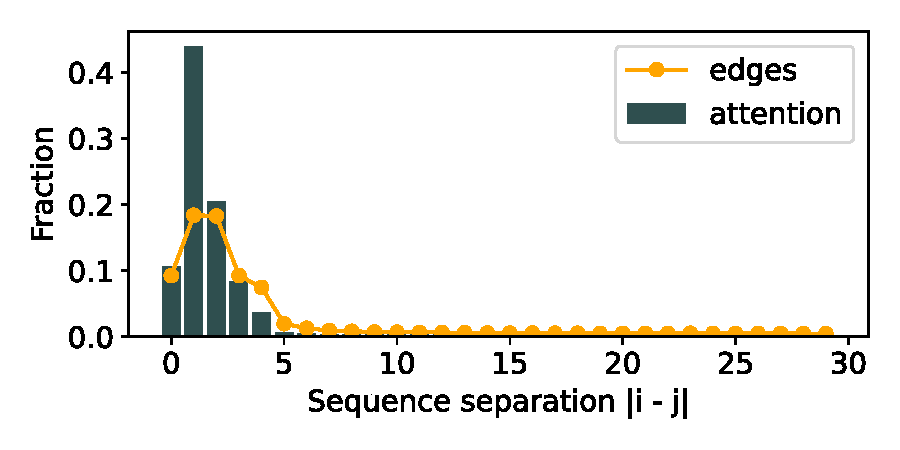
\includegraphics[width=0.6\textwidth]{figures/attention_by_separation.pdf}
\caption{Share of attention in the last GATv2 layer (bars) and share of edges (line) by sequence separation, over 500 test proteins.}
\label{fig:att}
\end{figure}

\section{Discussion}\label{sec:discussion}

\paragraph{Lessons for graph learning.} First, evaluation choices can change conclusions. A random split would have made GCN appear better than a tree model, and the inflation differs across model classes, so leakage cannot be treated as a constant offset. Second, node input design can matter more than architecture. On a graph with no attributes, the input added 6--7 points for every model, as much as the gap between GCN and the attention models. Third, uninformative inputs can cause failures that the architecture does not reveal. The collapse of attention with constant inputs follows from the use of edge features in the attention coefficients only, and it would apply to other attribute-free graphs. Fourth, wider models were not better here, and small attention models were enough.

\paragraph{PSS-net as a reference model.} Among the models tested, PSS-net combines the best accuracy with the smallest size among selected models and a low spread across seeds, 0.03 points against 0.05--0.19 for the other GNNs run with several seeds. Along with GAT, it is the most tolerant of spurious edges. Among the three GNNs compared on both splits, it gains the least from a random split. Its weaknesses are its training time and its sensitivity to missing short-range contacts.

\paragraph{Possible uses.} Beyond benchmarking, contact maps are an important representation of proteins: they retain enough information to recover the fold~\cite{vendruscolo1997recovery} and can be predicted from coevolution~\cite{morcos2011direct}. Models like these could read local structure from predicted maps or from contact-like experimental data, and their representations could serve downstream tasks. We have not validated these uses, and our robustness results suggest they would need training on noisy or sparse maps.

\paragraph{Limitations.}
\begin{itemize}
    \item The contact-separation input was developed during preliminary runs on this split, whose test scores we saw, and $R$ was not tuned. Its gain is large compared with any plausible selection effect, but the absolute accuracy of the best model may be slightly optimistic. Future comparisons should follow the protocol strictly.
    \item The 30\% identity split removes close homologs, but remote homologs with the same fold can remain across the split. A fold-level split based on CATH or SCOP would be stricter.
    \item Labels are PDB records and vary across sources. Boundaries are their least well-defined part, as the disagreement with DSSP shows, so part of the residual error may reflect label noise.
    \item Only one chain is used, so sheets that pair across chains appear without their partner strands. The dataset has no quality filter and includes entries with the same sequence.
    \item Robustness was measured by perturbing edges, not by rebuilding graphs at another threshold.
    \item Input, leakage, and robustness experiments use one seed. Since residues within a protein are not independent, we report variation across seeds and do not report significance tests.
\end{itemize}

\section{Conclusion}\label{sec:conclusion}

We introduced GraphPSS, a large inductive node classification benchmark of 173K protein contact graphs, with a homology-aware split, an evaluation protocol, and reference baselines. PSS-net, a compact attention model, sets the baseline at 91.02\% with 1.7M parameters. The results show that leakage can inflate GNN accuracy and change model rankings, that node input design can outweigh architecture on attribute-free graphs, and that expanding the neighborhood benefits graph convolution. We hope GraphPSS helps future graph learning methods to be evaluated at scale and on realistic generalization.

\backmatter

\section*{Declarations}

\begin{itemize}
    \item \textbf{Funding:} The author received no specific funding for this work.
    \item \textbf{Competing interests:} The author has no competing interests to declare.
    \item \textbf{Data availability:} The GraphPSS graphs and splits are available on Zenodo at \url{https://doi.org/10.5281/zenodo.23829544}. The underlying structures are available from the Protein Data Bank.
    \item \textbf{Code availability:} The code is available at \url{https://github.com/ialireza13/graphpss}.
    \item \textbf{Author contribution:} A.H. designed the study, curated the dataset, conducted the experiments, and wrote the manuscript.
    \item \textbf{Use of AI tools:} The author used Claude (Anthropic) to assist with code development, experiment execution, data analysis, and drafting and editing the manuscript. The author reviewed the results and text and takes full responsibility for the content.
\end{itemize}

\bibliography{references}

\end{document}
